\documentclass{article}

% if you need to pass options to natbib, use, e.g.:
% \PassOptionsToPackage{numbers, compress}{natbib}
% before loading nips_2016
%
% to avoid loading the natbib package, add option nonatbib:
% \usepackage[nonatbib]{nips_2016}

%\usepackage{nips_2016}

% to compile a camera-ready version, add the [final] option, e.g.:
% \usepackage[final]{nips_2016}

\usepackage[utf8]{inputenc} % allow utf-8 input
\usepackage[T1]{fontenc}    % use 8-bit T1 fonts
\usepackage[hidelinks]{hyperref}       % hyperlinks
\usepackage{url}            % simple URL typesetting
\usepackage{booktabs}       % professional-quality tables
\usepackage{amsfonts}       % blackboard math symbols
\usepackage{nicefrac}       % compact symbols for 1/2, etc.
\usepackage{microtype}      % microtypography
\usepackage{amsmath}
\usepackage{cleveref}
\usepackage{csvsimple}
\usepackage{graphicx}
\usepackage{color}

\title{Feature Selection in Finance, It is Delicious}
\usepackage[final]{nips_2016}

% The \author macro works with any number of authors. There are two
% commands used to separate the names and addresses of multiple
% authors: \And and \AND.
%
% Using \And between authors leaves it to LaTeX to determine where to
% break the lines. Using \AND forces a line break at that point. So,
% if LaTeX puts 3 of 4 authors names on the first line, and the last
% on the second line, try using \AND instead of \And before the third
% author name.

\author{
  Benjamin A. Schifman\\
  \textbf{Justin J. Siekmann}\\
  Department of Electrical and Computer Engineering\\
  University of Arizona\\
  Tucson, AZ 85719 \\
  \texttt{bschifman@email.arizona.edu} \\
  \texttt{jsiekmannemail.arizona.edu}
}

\begin{document}
 

\maketitle

\begin{abstract}
	\color{red}
  The abstract paragraph should be indented \nicefrac{1}{2}~inch
  (3~picas) on both the left- and right-hand margins. Use 10~point
  type, with a vertical spacing (leading) of 11~points.  The word
  \textbf{Abstract} must be centered, bold, and in point size 12. Two
  line spaces precede the abstract. The abstract must be limited to
  one paragraph.
\end{abstract}

\section{\color{red}Introduction}
There exist technical analysis indicators traditionally used by analysts to evaluate and predict market and equity performance, as they “can provide a unique perspective on the strength and direction of the underlying price action” ({\bf <--what is this quote from??}). \\
Feature selection is used to determine relevant indicators while identifying those that are irrelevant and redundant. Different implementations of algorithms based on these indicators could be used to predict performance of individual equities, sectors, or overall markets. They could also be used to classify and identify the correlation and interdependencies between equities, sectors, and markets. Our goal is to implement various approaches to determine efficacy of technical indicators as enablers to financial analysis. This project presented a couple challenges during implementation including developing an accurate testing method as well as handling and computing such large volumes of data.

Possibly reword and keep/move:\\
From this project we hope to deepen our understanding of the usage cases for applying specific machine learning algorithms as well as expanding upon our technical analysis of the stock market and which indicators play a role in successful market analysis.

\section{Related Work}
This is optional. If wanted, save til last.

\section{Methods/Approach}
The following subsections present details and explanations of the methods and functions implemented as part of this project.

\subsection{Data and Technical Analysis Indicators}
The Quandl platform was used to fetch 11 years of market data from Dec 31, 2006 to Dec 31, 2017 on various identified US tickers across different sectors. Tickers used in the project can be found in Table \ref{tab:tick} categorized by sector. As the amount of fetched and calculated data is very large, pickle files were used to save all data to be quickly reimported instead of refetching data through the Quandl platform. TA-Lib: Technical Analysis Library was used to calculate features on the market data for each ticker obtained using Quandl. <insert stuff about TA-lib having various types of features>. The features incorporated into this project are found with in \Cref{tab:inds}.

\begin{table}[h]
	\centering
	\csvautotabular{data/tickers.csv}
	\caption{Tickers}
	\label{tab:tick}
\end{table}

\begin{table}[h]
	\csvreader[respect all, autotabular]{data/features.csv}{}{\csvlinetotablerow}
	\centering
	\caption{Technical Analysis Indicators}
	\label{tab:inds}
\end{table}

\subsection{Normalization}
As each technical analysis indicator produces values applicable based on the way the indicator was calculated, normalization of the indicators makes correlations between them during feature selection more accurate and applicable. Each value in a specified time period is normalized using Equation \eqref{eq:norm}. If there is extra data not consisting of a full time period, the extras are thrown out at the beginning of the data as data near the end may be more relevant and thus more desirable to keep. The start indices are computed for each ticker and return to ease future handling.

\begin{equation}\label{eq:norm}
	x_n = \frac{x - min}{max - min}
\end{equation}

\subsection{Feature Correlation}
Removing highly correlated features allows for the optimization of the classification algorithms by reducing the feature space. Features that are highly correlated most likely offer no additional data and they are an extra expense in computation time. The pairwise correlation of columns was computed, and columns that were correlated above a certain threshold were marked to be removed from future classification algorithms. The following Figure~\ref{fig:corr_heatmap}

\begin{figure}[h!]
	\centering
	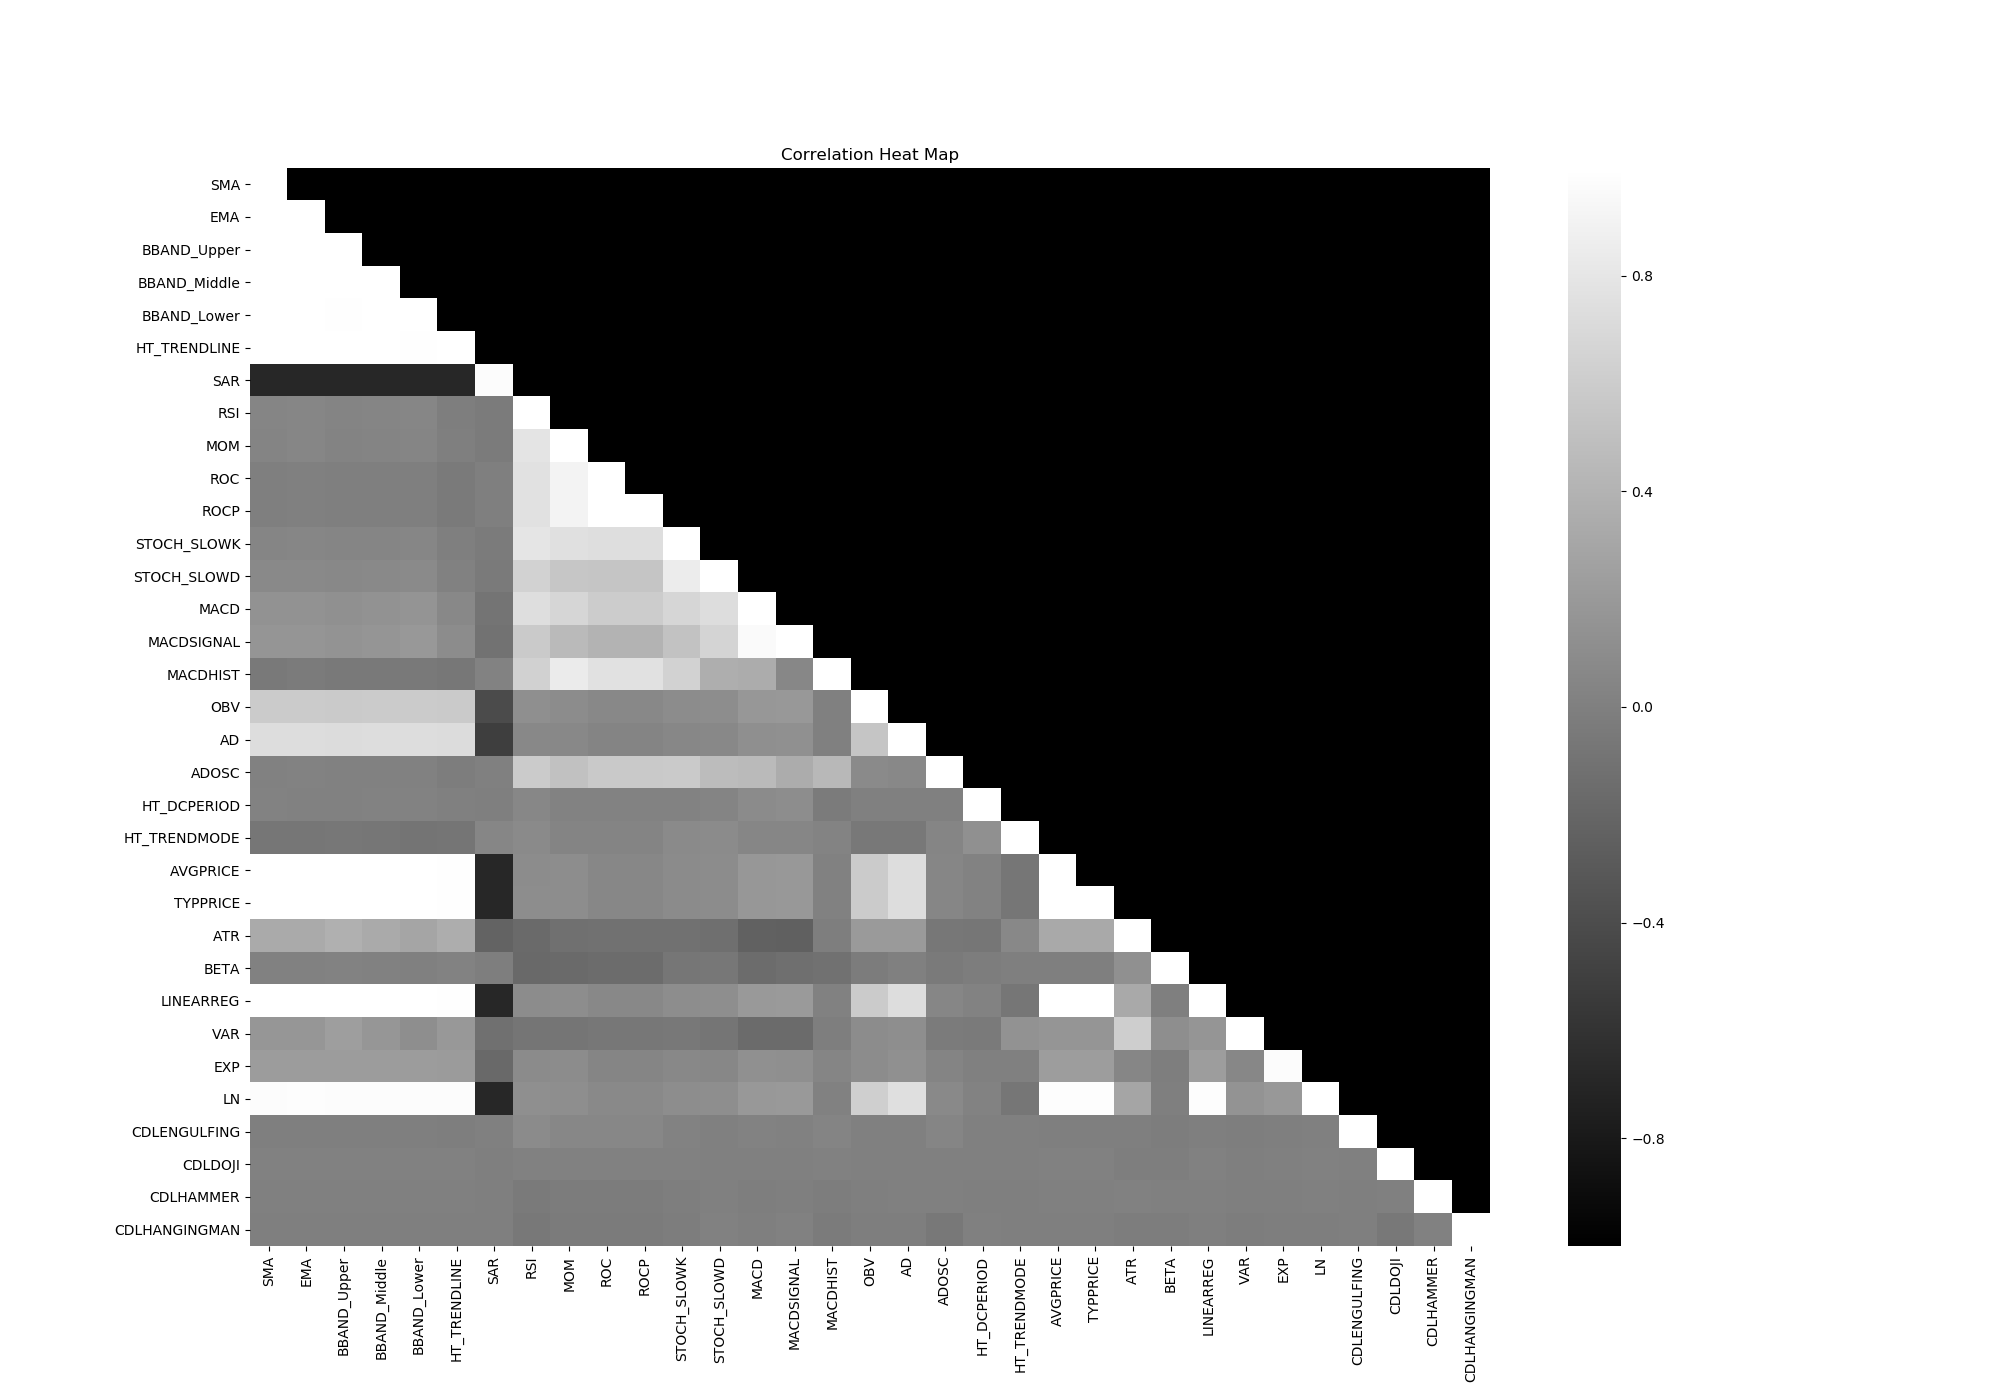
\includegraphics[width=\linewidth]{data/heatmapT1.png}
	\caption{Heat Map of Correlated Variables}
	\label{fig:corr_heatmap}
\end{figure}

\subsection{Maximal Information Coefficient (MIC)}
The MIC is "a measure of two-variable dependence designed specifically for rapid exploration of many-dimensional data sets" - http://www.exploredata.net/. A benefit to MIC correlations between two variables is that it can be described regardless of linear or non-linear relationships. The MIC yields a single vale $0 \leq MIC \leq 1$ with a value closer to $1$ representing that the variables are more closely correlated, and a value near $0$ indicates statistically independent variables that have neither linear nor nonlinear relationships. The $minepy$ library was used in python to rank the features according to their MIC with the target variable. The MIC was calculated for each feature in each ticker, and then a final MIC value for each feature was calculated by taking the mean of the values.

\textbf{\color{red}ADD TABLE OF MIC RESULTS!}

\subsection{\color{red}Recursive Feature Elimination (RFE)}
Given an external estimator 


\subsection{\color{red}Random Forest Classifier (RFC)}
The Random Forest Classifier is an ensemble technique implementing decision trees and 


\subsection{\color{red}Principle Component Analysis (PCA)}
PCA orthogonally transforms a set of features into a set of linearly uncorrelated principal components. PCA is a method for reducing the dimensionality of the feature set size while retaining principal component variance, and the features informational relevance. To analyze the performance of this method, PCA was implemented on the original 33 features and then the resulting principal components were used in the RFC classifier with 5 fold cross validation to see the resultant accuracy. The number of principal components were iterated from 1 to 33 and then the principal component were implemented in the RFC to find the optimal number of principal components to yield the best accuracy and in the least amount of time.  

\begin{table}[h]
	\csvreader[respect all, autotabular]{data/PCAT1.csv}{}{\csvlinetotablerow}
	\centering
	\caption{Principal Component Analysis}
	\label{tab:pca}
\end{table}


\section{Results}
\section{Conclusion}

\section*{References}


\end{document}